\documentclass[a4paper]{book}
\usepackage{tocbibind} % for toc show inside pdf
\usepackage[
	%urlbordercolor = {1 1 1},
	%linkbordercolor = {1 1 1},
	%citebordercolor = {1 1 1},
    bookmarksnumbered, % add bookmark number in pdf output
	urlcolor = blue,
	colorlinks = true,
	citecolor = black,
	linkcolor = black]{hyperref}
\usepackage{graphicx}
\usepackage{xltxtra}
\usepackage{fancyhdr}
\usepackage{booktabs}
\usepackage{indentfirst}
\usepackage{framed,color}
\usepackage{footnpag}
\usepackage{array}
\usepackage[font=small,format=plain,labelfont=bf,up,textfont=it,up]{caption}

\usepackage{titlesec} % texlive-latex-extra package
\usepackage[titletoc]{appendix} % this is used for \appendices

\definecolor{colorchapter}{RGB}{70,130,180}     % SteelBlue
\definecolor{colorsection}{RGB}{95,158,160}    % CadetBlue
\definecolor{colorsubsection}{RGB}{139,0,0} % DarkRed
\definecolor{colorheader}{RGB}{70,130,180} % SteelBlue


\titleformat{\section}
{\color{colorsection}\normalfont\Large\bfseries}
{\color{colorsection}\thesection}{1em}{}
\titleformat{\subsection}
{\color{colorsubsection}\normalfont\large\bfseries}
{\color{colorsubsection}\thesubsection}{1em}{}

\definecolor{shadecolor}{gray}{0.90}

\setromanfont[Mapping=tex-text,BoldFont=WenQuanYi Micro Hei]{AR PL SungtiL GB}
\setmonofont{WenQuanYi Zen Hei Mono}

\XeTeXlinebreaklocale{zh}
\XeTeXlinebreakskip=0em plus 0.1em minus 0.01em
\XeTeXlinebreakpenalty=0

\settowidth{\parindent}{文文}
\setcounter{footnote}{0}

\title{{跟我学STM8}}
\author{Larry Cai}

\makeatletter
\let\savedauthor=\@author
\let\savedtitle=\@title
\def\imgwidth{.6\linewidth}
\def\maxwidth{\ifdim\Gin@nat@width>\imgwidth\imgwidth
\else\Gin@nat@width\fi}
\makeatother

\title{\huge{\savedtitle}}

\author{\textbf{\savedauthor}\thanks{}}
\def\w3cdtfymd{\the\year-\ifnum\month<10 0\fi\the\month-\ifnum\day<10 0\fi\the\day}
\date{\w3cdtfymd}
%\renewcommand{\thefootnote}{\fnsymbol{footnote}}

\newcommand{\PreserveBackslash}[1]{\let\temp=\\#1\let\\=\temp}
\let\PBS=\PreserveBackslash
\makeatletter
  \setlength\headheight{12\p@}
  \setlength\headsep   {.25in}
  \setlength\topskip   {10\p@}
  \setlength\footskip{.35in}
  \setlength\textwidth{400\p@}
  
  \setlength\@tempdima{\paperheight}
  \addtolength\@tempdima{-2in}
  \divide\@tempdima\baselineskip
  \@tempcnta=\@tempdima
  \setlength\textheight{\@tempcnta\baselineskip}
  \addtolength\textheight{\topskip}
  
  \setlength\@tempdima        {\paperwidth}
  \addtolength\@tempdima      {-\textwidth}
  \setlength\oddsidemargin    {\paperwidth}
  \addtolength\oddsidemargin  {-2.35in}
  \addtolength\oddsidemargin  {-\textwidth}
  \setlength\marginparwidth   {0pt}
  \@settopoint\oddsidemargin
  \@settopoint\marginparwidth
  \setlength\evensidemargin  {\paperwidth}
  \addtolength\evensidemargin{-2.35in}
  \addtolength\evensidemargin{-\textwidth}
  \@settopoint\evensidemargin
  
  \setlength\topmargin{\paperheight}
  \addtolength\topmargin{-2in}
  \addtolength\topmargin{-\headheight}
  \addtolength\topmargin{-\headsep}
  \addtolength\topmargin{-\textheight}
  \addtolength\topmargin{-\footskip}     % this might be wrong!
  \addtolength\topmargin{-.5\topmargin}
  \@settopoint\topmargin
  %\@addtoreset{footnote}{page}  
\makeatother

%\fancypagestyle{plain}{\fancyhf{}\fancyfoot[LE,RO]{\footnotesize\textbf\thepage}}
\fancypagestyle{plain}{\fancyhf{}\fancyfoot{}} % make sure no page number in page of first chapter

\pagestyle{plain}


\renewcommand{\headrulewidth}{0pt}
\renewcommand{\footrulewidth}{0pt}

\newcounter{img}[chapter]
\renewcommand{\theimg}{\thechapter.\arabic{img}}
\newcommand{\img}[1]{\begin{figure}[h!]
	\refstepcounter{img}
	\label{img:\theimg}
	\centering\includegraphics[width=\maxwidth]{figures/\theimg.png}
	\caption{#1}
\end{figure}}

\newcounter{tab}[chapter]
\renewcommand{\thetab}{\thechapter.\arabic{tab}}

\newcommand{\prechap}{第}
\newcommand{\postchap}{章}
\newcommand{\presect}{}
\newcommand{\postsect}{节}
\renewcommand{\chaptermark}[1]{\markboth{\textbf{\prechap \thechapter \postchap}\hspace*{1ex}#1}{}}
\renewcommand{\sectionmark}[1]{\markright{\textbf{\presect \thesection \postsect}\hspace*{1ex}#1}}
\newcommand{\chap}[1]{\newpage\thispagestyle{empty}\chapter{#1}\label{chap:\thechapter}}
\newcommand{\chapref}[1]{\hyperref[chap:#1]{\prechap #1\postchap}}
\newcommand{\imgref}[1]{\hyperref[img:#1]{图 #1}}
\newcommand{\tabref}[1]{\hyperref[tab:#1]{表 #1}}
\newcommand{\e}[1]{$ \times 10^{#1}$}
\renewcommand{\contentsname}{目录}
\renewcommand{\figurename}{图 }
\renewcommand{\tablename}{表 }
\renewcommand{\appendixname}{}

% chapter 
\makeatletter
\def\@makechapterhead#1{%
  \vspace*{50\p@}%
  {\parindent \z@ \raggedright \normalfont
    \ifnum \c@secnumdepth >\m@ne
      \if@mainmatter
        \color{colorchapter}\normalfont\huge\bfseries\prechap{ }\thechapter{ }\postchap
        \par\nobreak
        \vskip 20\p@
      \fi
    \fi
    \interlinepenalty\@M
    \color{colorchapter}\normalfont\Huge\bfseries #1\par\nobreak
    \vskip 40\p@
  }}  
 
% this is for non-normal chapter like Acknownledgement, Preface, Contents  
\def\@makeschapterhead#1{%
  \vspace*{50\p@}%
  {\parindent \z@ \raggedright \normalfont
    \ifnum \c@secnumdepth >\m@ne
      \if@mainmatter
        \color{colorchapter}\normalfont\huge\bfseries \thechapter{ }
        \par\nobreak
        \vskip 20\p@
      \fi
    \fi
    \interlinepenalty\@M
    \color{colorchapter}\normalfont\Huge\bfseries #1\par\nobreak
    \vskip 40\p@
  }}  
\makeatother

\linespread{1.3}

\begin{document}
%\maketitle
\thispagestyle{empty}
\setcounter{tocdepth}{4}

\frontmatter
\chapter*{前言}
\addcontentsline{toc}{chapter}{前言}

说起这本手册的起因,是我去年6月做项目时上时碰到STM8这块芯片。这块芯片性能很强大,但是缺少对应的教材。当时我全靠着ST的英文文档,看得比较累。空下来就想,如果能有本教材就好了。毕设选题时,因为自己也做过一些研发类的项目,想换种形式,想到了这件事,就决定干脆自己写本教材。 但最后决定写成手册的形式,是因为一篇大牛的博客。这位大牛自身的技术积淀已经很强了,网上最流行的中文makefile教程就是他写的。他写的博文我经常看,感觉很有深度。据说很多出版社找他请他出书,但是他拒绝了,他说了这么一句话:“45岁之前绝不出书”,因为他觉得只有到了那个时候,自己才可能得到足够的积淀,才可能出的了精品。看到这句话,我非常惭愧,红着脸把“书”改成“手册”了。 在惠普以及爱立信的实习过程中,我接触了很多软件方面好用的工具,成熟的软件工程思想。比如说git,就是非常好的版本控制管理软件,比如说agile,消除了传统软件开发过程中的部分问题。我觉得,软件开发中的诸多问题,随着编程规模的扩大,参与人数的增多,在硬件开发中也会逐步地体现出来。所以,这些工具及思想方式引入到嵌入式编程,将是一种趋势。本手册亦不指望能够引领什么潮流,只希望能对STM8的学习者,有一个有益的指导,仅此而已。

\subsection*{适合的对象}

本手册适合具有C语言功底,并能在51或AVR上进行简单程序设计的单片机爱好者。如果没有C语言基础的,推荐\href{http://product.china-pub.com/14975\&ref=browse}{《C程序设计语言》},没有单片机基础的,本手册建议从马潮教授编写的\href{http://www.amazon.cn/AVR\%E5\%8D\%95\%E7\%89\%87\%E6\%9C\%BA\%E5\%B5\%8C\%E5\%85\%A5\%E5\%BC\%8F\%E7\%B3\%BB\%E7\%BB\%9F\%E5\%8E\%9F\%E7\%90\%86\%E4\%B8\%8E\%E5\%BA\%94\%E7\%94\%A8\%E5\%AE\%9E\%E8\%B7\%B5-\%E9\%A9\%AC\%E6\%BD\%AE/dp/B005GZQWB0/ref=sr\_1\_1?ie=UTF8\&qid=1335097650\&sr=8-1}{《AVR单片机嵌入式系统原理与应用实践(第2版)》}

\section*{本书结构}

\begin{itemize}\setlength{\itemsep}{1pt}\setlength{\parskip}{0pt}\setlength{\parsep}{0pt}
\item[*]
  第一章:前言
\item[*]
  第二章:重读C语言
\item[*]
  第三章:软件开发那点事
\item[*]
  第四章:STM8芯片资源简介
\item[*]
  第五章:STM8官方软件库简介
\item[*]
  第六章:STM8S编程实战
\end{itemize}
\subsection*{封面及封底}

因为自己喜欢排版,就自己设计了一个。封面封底的图片都是取景自华师大校园的风景,本手册封面、封底都是使用COREDRAW设计的。

\subsection*{项目地址}

本次STM8学习项目托管在github上,并且项目完全开源。欢迎大家访问:\href{www.github.com/vincent5295/stm8teach}{www.github.com/vincent5295/stm8teach}

\section*{如何写作本手册的}

本手册是使用MARKDOWN格式写作的,感谢larrycai的\href{www.github.com/larrycai/mkbok}{mkbok项目}。

\subsection*{你不能从本手册中获得}

本手册不是官方数据手册的汉化并堆砌,故详细的硬件寄存器资源及软件库函数说明并不能从中得到。手册本身不需实现盈利,故针对某开发板的内容在手册上也不能获得。同样关于程序语言的章节也不会提供过多C语言的细节。但以上这些在相关章节都会提到相应资源的方法,并且提供经验上的参考。

\subsection*{如何阅读本手册}

一般来说,建议直接阅读电子版,一来可以获得较好的阅读体验,二来可以节约纸张。从保护视力的角度出发,自行打印纸质版也是可以的。但请一定不要忽视电子版,文中随处的可见的链接,是一笔宝贵的财富。本手册编写的一大准则,就是以自身为骨架,通过这些链接,能让读者得到丰富的内容。

\subsection*{项目网站上的开发板}

项目网站上的核心板、资源板基于开放式设计。只是一个参考,如果不愿意自己画板子,可以直接将网站上的板子发到制版厂做,或者在网上买一款开发板都是可行的。资源板只提供原理图(因为模块太多,都做板子不实惠),因为这些模块PCB设计比较简单,需要做PCB的,自行copy所需模块,导入至PCB文件,连少许线即可。

\section*{致谢}

在本手册的编写过程中,遇到很多困难。在此感谢惠普以及爱立信的同事在软件编程方面对我的指点。特别要感谢爱立信中国通讯有限公司为期一周的敏捷开发培训,学到了不少有趣的东西。感谢larrycai在Github上的\href{www.github.com/larrycai/kaiyuanbook}{kaiyuanbook}以及\href{www.github.com/larrycai/mkbok}{mkbok}项目,为本手册的快速写作奠定了基础。最后要感谢周围的老师同学们在本项目的实践过程中,对本人给予的无私帮助,正是有了你们的鼓励与支持,才能有这个项目。

\tableofcontents\newpage\thispagestyle{empty}

% customize header & footer

\fancyhf{}
\fancyhead[LE]{\color{colorheader}\quad\small\textbf\thepage\quad\quad\small\leftmark}
\fancyhead[RO]{\color{colorheader}\small\rightmark\quad\quad\small\textbf\thepage\quad}
%\fancyhead[RE,LO]{\color{colorheader}\small{\savedtitle}} % book title 
%\fancyfoot[LE,RO]{\small\textbf\thepage} % page number
%\fancyfoot[C]{\small\textbf{hello}} % could add release information

%\renewcommand{\headrulewidth}{0.4pt}  % add one line
%\renewcommand{\headrule}{\color{red}} % conflict with headrulewidth
\pagestyle{fancy}

\mainmatter
\chap{重读C语言}

\section{一个小测试}

说到C语言,可能你还不以为然。这个语言是众多学院的编程入门语言,似乎当年写的几个程序还挺简单的。那么来做一下下面几个测试,看看自己C语言到底学的怎么样吧!

如果不过瘾的话,\href{http://coolshell.cn/articles/945.html}{这里},还有\href{http://coolshell.cn/articles/873.html}{这里},都可以让你比较深入的去思考,同时相信类似的这些问题在你今后找工作的面试中一定碰得到,除非你不做程序员。 这些

关于进一步学习C语言的资料,我这里推荐下列三本书:\href{http://product.china-pub.com/14975\&ref=browse}{《C程序设计语言》}、{[}《C专家编程》{]}http://product.china-pub.com/38005)、\href{http://product.china-pub.com/38125}{《C陷阱与缺陷》}。一般来说,以《C程序设计语言》为基础,然后凭借后面两本书,知道C语言平时使用中一些容易犯错的地方。当然,如果你觉得还不够的话,以下这篇文章可能会适合你:\href{http://coolshell.cn/articles/4102.html}{如何学好C语言}。

\chap{软件开发那点事}

下面是一些开发方面的问题:你有没有使用vim写过一个50行以上的小程序?你有没有使用过gcc编译,再用gdb调试过程序?你有没有写过一个makefile,写好程序后敲一个make,编译、测试、安装或者更多的东西一键搞定。当然如果作为大的软件项目来说,版本控制系统自然是少不了的,那么你有没有使用过Git、CVS或是SVN,对项目的代码checkin、checkout、merge、revert?

\section{使用GitHub来管理你的项目}

\chap{STM8芯片简介}

\section{STM8的优势}

STM8S是意法半导体推出的一款8位高性能单片机。它基于哈弗结构,指令与数据存储空间分开,指令与数据可以同时存取,因而具有更高的执行效率。与AVR、51单片机比较,STM8拥有更为丰富的外设,更强大的主频、更优秀的特性。更重要的是,STM8供货稳定,性价比高。其中高端的STM8S208MB也就15元,低端的STM8S103F2系列一般也就2、3元左右,而AVR高端的mega128价格就在20元左右,且性能只能勉强赶得上ST的中端产品。更重要的是,STM8的编程方法与ST的高端产品,cortexM3市场的主流:STM32极其相似(但更简单点)。这种相似,给我们后来升级到STM32奠定了基础,要知道STM32最高端的F4系列具有150Mhz的主频,这样的升级,可以大大提升我们以后做应用的范围。

\section{STM8编程------寄存器or库函数?}

和STM32一样,历来STM8存在两种编程方式:寄存器直接编程和库函数编程。寄存器的优势在于,这样的编程方法和传统的8位单片机编程方法较一致,初学者容易适应,而且普遍认为寄存器编程的人不容易出错,程序执行效率较高。库函数的优势在于程序员开发效率高,ST将一些常用的方法封装起来,这样寄存器开发者几句话(可能还得经常查手册找参数)才能搞定的事情,库函数直接一个函数就搞定了,而且所有的参数设定都可以在库函数附带的使用手册中找到,方便快捷。 事实上,因为开发效率在实际应用中往往起着决定性的作用,比如大家同样做一个新产品,只有第一个做出来的才能在很早的时候抢占市场。等市场有了,在对产品维护的过程中优化程序运行效率。同时,使用库函数的方式能更好适应以后STM32,甚至DSP、ARM的编程方式。基于上述两个原因,本手册建议使用库函数编程方式。

\section{芯片资源简介}

一般来说,学习的时候可以用芯片功能强大一点,具体开发产品的时候可以根据官方给的\href{http://www.st.com/internet/com/SALES\_AND\_MARKETING\_RESOURCES/MARKETING\_COMMUNICATION/MARKETING\_BROCHURE/brstm8.pdf}{选型指南},来选择对应的芯片。本手册选用的是STM8S208MB芯片,它具有: \emph{最大24Mhz的运行速率}80个引脚(其中68个可用作IO引脚) \emph{37个外部中断引脚}128K可编程Flash,2MB的EEPROM \emph{6KB的RAM}并拥有CAN总线接口\ldots{}\ldots{} 具体资源可以从STM8S208MB的\href{http://www.st.com/internet/com/TECHNICAL\_RESOURCES/TECHNICAL\_LITERATURE/DATASHEET/CD00197787.pdf}{数据手册}获取,该芯片的APPLICATION NOTES、PROGRAMMING MANUALS、REFERENCE MANUALS等信息,可以从\href{http://www.st.com/internet/mcu/product/190232.jsp}{芯片的主页}下载。

\begin{figure}[htbp]
\centering
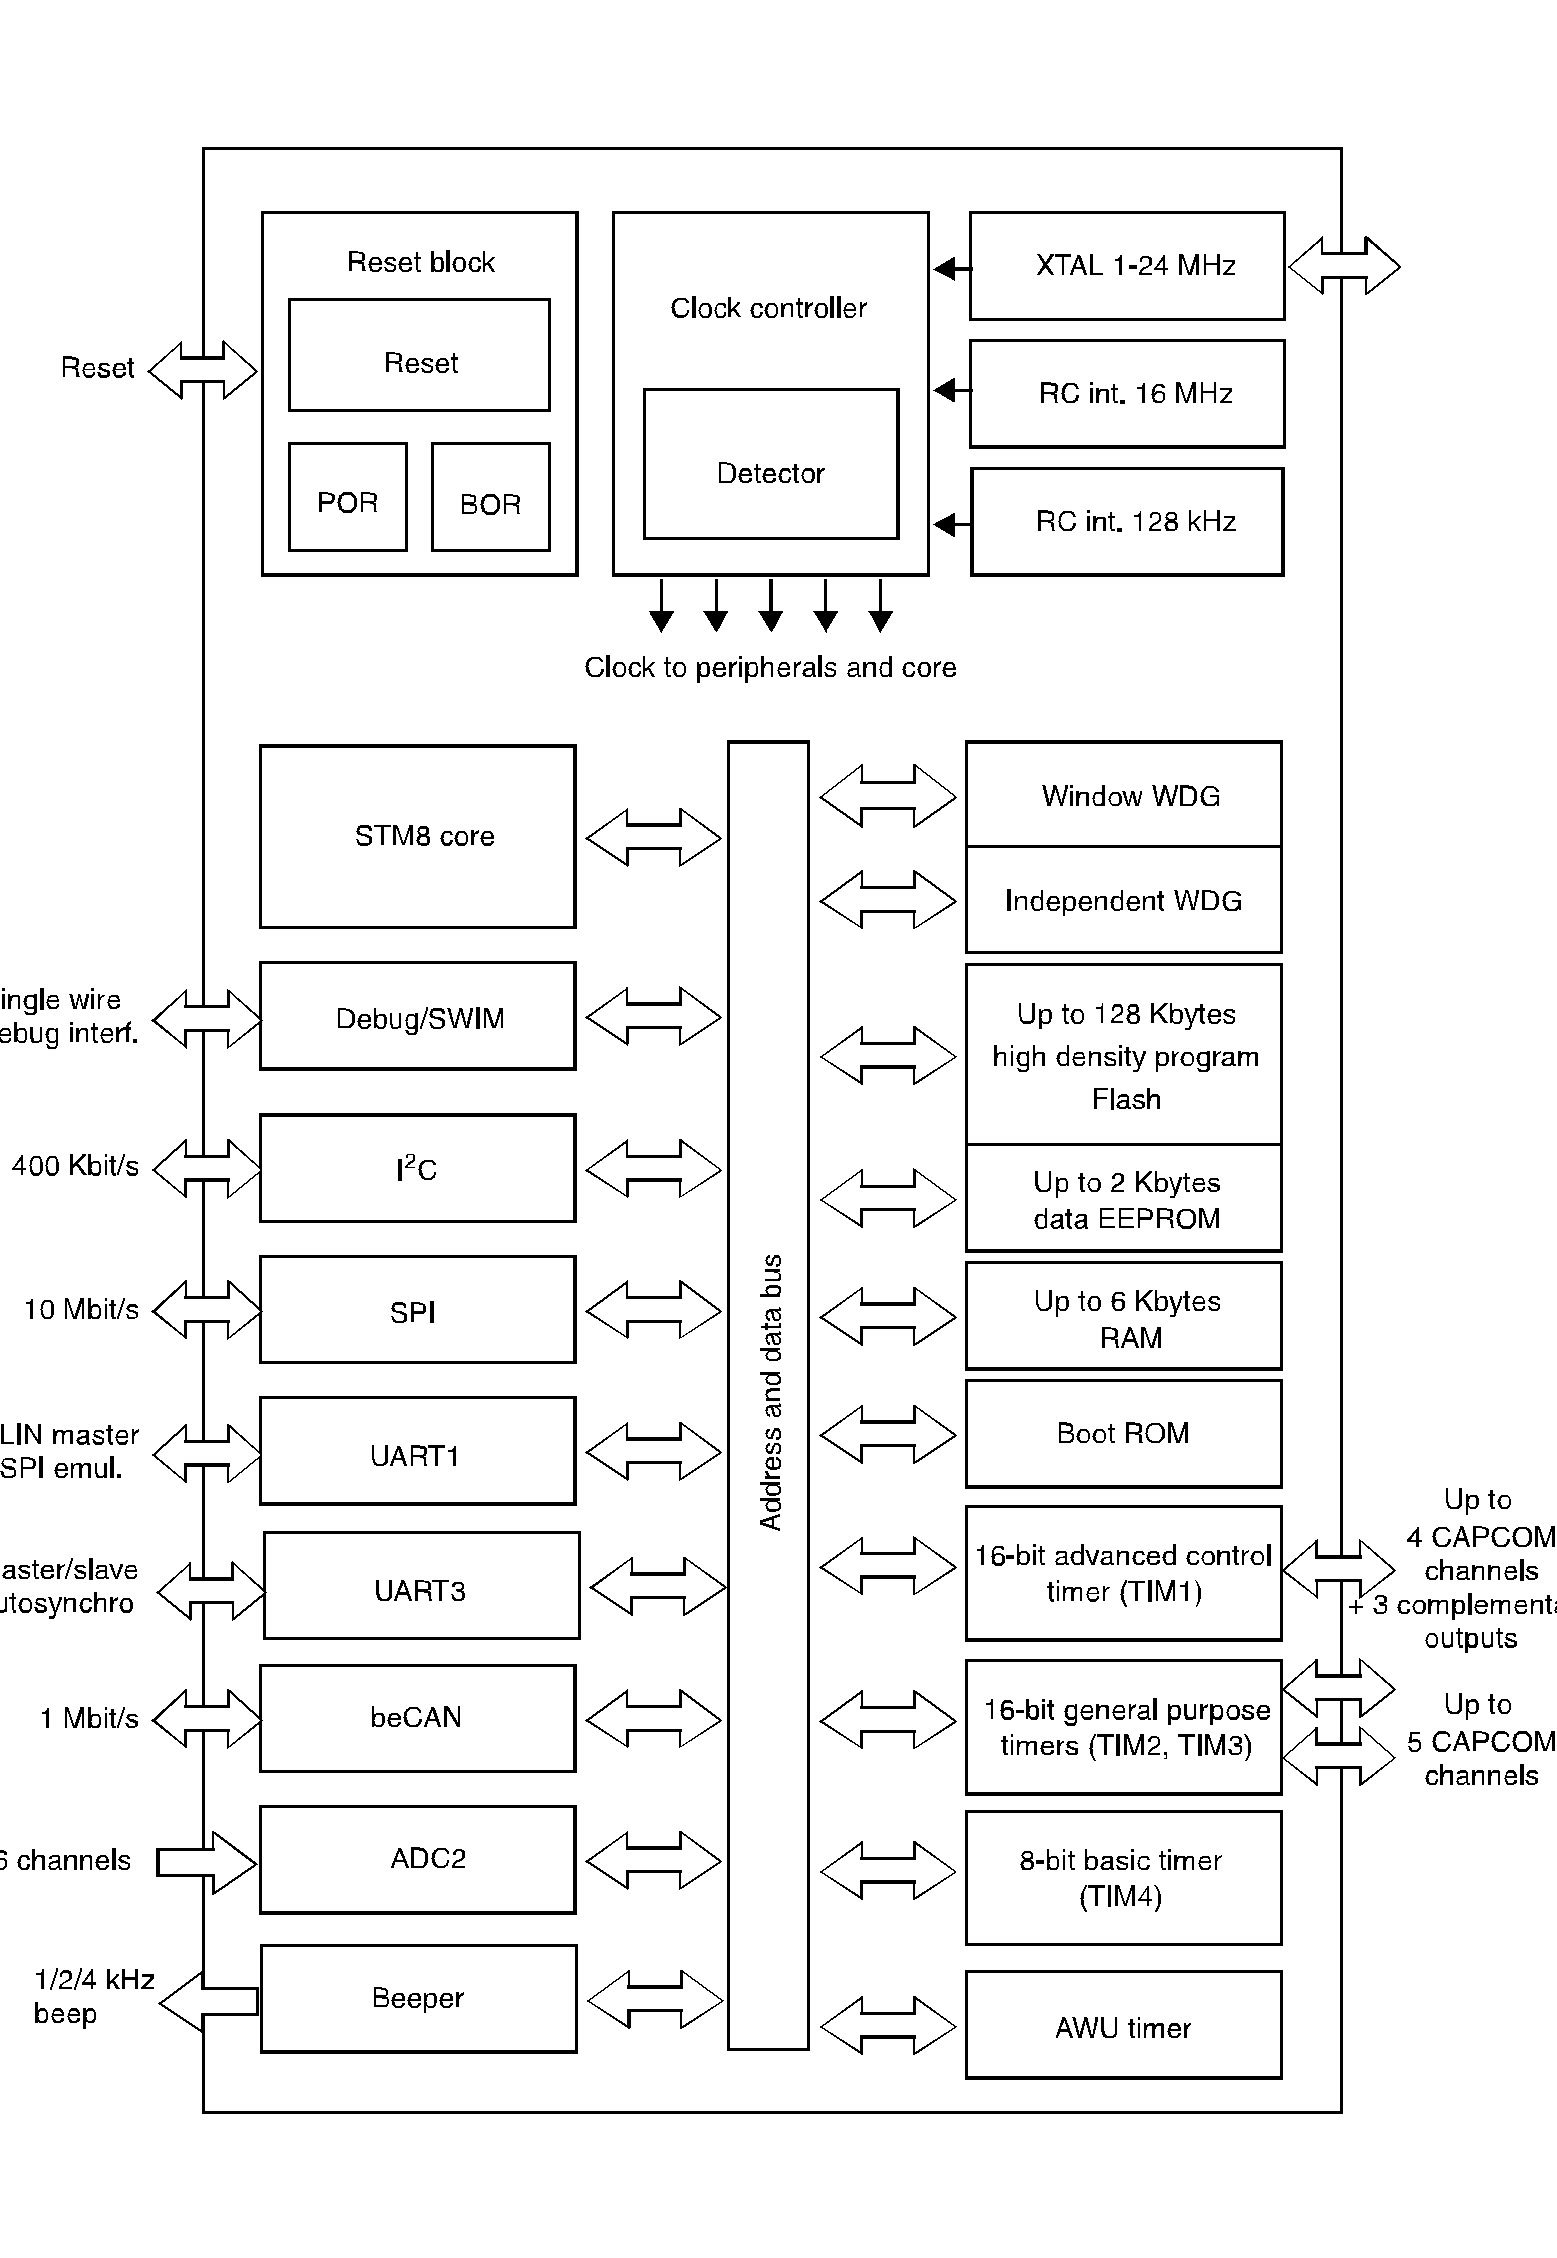
\includegraphics{figures/circuit_diagram.jpg}
\caption{芯片的电路图}
\end{figure}

\chap{STM8官方软件库简介}

\chap{STM8编程实战}

\section{实验一跑马灯}



\appendices
\renewcommand{\prechap}{\appendixname}
\renewcommand{\postchap}{}


\end{document}
